\section{arXiv Paper Domain Classification}
\label{appendix:domain_mapping}
We use the \href{https://arxiv.org/category_taxonomy}{arXiv category taxonomy}. Since Computer Science has many subfields, we further group the arXiv category labels into broader macro-domains.
\begin{table}[htbp]
\centering
\resizebox{\textwidth}{!}{%
\begin{tabular}{ll}
\toprule
\textbf{Domain} & \textbf{arXiv Labels} \\
\midrule
Language & cs.CL \\
ML/AI & cs.LG, cs.AI, cs.NE, cs.MA \\
Robotics & cs.RO \\
Vision & cs.CV, cs.GR, cs.MM, cs.SD \\
Theory & cs.CC, cs.DS, cs.FL, cs.LO, cs.DM, cs.CG, cs.GT, cs.CR, cs.IT \\
Systems & cs.AR, cs.OS, cs.DC, cs.NI, cs.PF, cs.SY, cs.PL, cs.SE, cs.DB, cs.IR, cs.SI \\
Society & cs.CY \\
HCI & cs.HC \\
CS-Other & cs.ET, cs.GL, cs.OH, cs.DL, cs.NA, cs.MS, cs.CE, cs.SC \\
Economics & econ \\
Electrical Engineering \& Systems Science (EE \& Sys. Sci.) & eess \\
Mathematics & math \\
Physics & astro-ph, cond-mat, gr-qc, hep-ex, hep-lat, hep-ph, hep-th, math-ph, nlin, nucl-ex, nucl-th, physics, quant-ph \\
Quantitative Biology (Quant. Bio.) & q-bio \\
Quantitative Finance (Quant. Fin.) & q-fin \\
Statistics & stat \\
\bottomrule
\end{tabular}%
}
\caption{Mapping from domains to arXiv category labels.}
\label{table:domain_mapping}
\end{table}



\section{Further Quantitative Analysis}

In this section, we provide a more granular, domain-by-domain breakdown of our quantitative results to better understand the performance characteristics of each model across different scientific disciplines. 

Table \ref{table:domain_results} presents the average similarity scores across the entirety of \ourbenchmark{}. The results demonstrate that \ourmethod{} achieves consistent, robust improvements over both the base models and the supervised fine-tuning (SFT) baselines. Notably, this performance gap holds steady across highly diverse fields, ranging from largely theoretical domains like Mathematics and Theory to applied disciplines such as Vision, Robotics, and HCI.

\begin{table}[htbp]
\centering
\resizebox{\textwidth}{!}{%
\begin{tabular}{lcccccc}
\toprule
\textbf{Domain} & \textbf{Base} & \textbf{SFT} & \textbf{SFT-think} & \textbf{\gemtwopro{}} & \textbf{\gemthreepro{}} & \textbf{\ourmethod{}} \\
\midrule
Economics & $4.66_{{\pm0.21}}$ & $4.78_{{\pm0.20}}$ & $4.94_{{\pm0.21}}$ & $4.75_{{\pm0.22}}$ & $4.50_{{\pm0.20}}$ & \textbf{$5.47_{{\pm0.22}}$} \\
Language & $4.50_{{\pm0.10}}$ & $4.75_{{\pm0.10}}$ & $4.84_{{\pm0.11}}$ & $4.45_{{\pm0.11}}$ & $4.14_{{\pm0.10}}$ & \textbf{$5.50_{{\pm0.11}}$} \\
Vision & $4.28_{{\pm0.10}}$ & $4.59_{{\pm0.10}}$ & $4.57_{{\pm0.10}}$ & $4.11_{{\pm0.10}}$ & $4.14_{{\pm0.10}}$ & \textbf{$5.52_{{\pm0.12}}$} \\
Theory & $4.54_{{\pm0.10}}$ & $4.72_{{\pm0.10}}$ & $4.80_{{\pm0.11}}$ & $4.67_{{\pm0.11}}$ & $4.58_{{\pm0.11}}$ & \textbf{$5.63_{{\pm0.11}}$} \\
Mathematics & $4.64_{{\pm0.11}}$ & $4.73_{{\pm0.10}}$ & $4.81_{{\pm0.10}}$ & $4.76_{{\pm0.11}}$ & $4.58_{{\pm0.10}}$ & \textbf{$5.66_{{\pm0.11}}$} \\
Quant. Fin. & $4.82_{{\pm0.25}}$ & $5.15_{{\pm0.23}}$ & $5.31_{{\pm0.25}}$ & $5.04_{{\pm0.26}}$ & $4.45_{{\pm0.24}}$ & \textbf{$5.75_{{\pm0.26}}$} \\
ML/AI & $4.77_{{\pm0.11}}$ & $4.97_{{\pm0.11}}$ & $4.87_{{\pm0.11}}$ & $4.64_{{\pm0.11}}$ & $4.56_{{\pm0.11}}$ & \textbf{$5.76_{{\pm0.12}}$} \\
Systems & $4.62_{{\pm0.11}}$ & $5.07_{{\pm0.11}}$ & $5.13_{{\pm0.11}}$ & $4.57_{{\pm0.11}}$ & $4.41_{{\pm0.11}}$ & \textbf{$6.04_{{\pm0.12}}$} \\
Society & $4.87_{{\pm0.14}}$ & $5.31_{{\pm0.14}}$ & $5.33_{{\pm0.15}}$ & $4.40_{{\pm0.13}}$ & $3.82_{{\pm0.11}}$ & \textbf{$6.05_{{\pm0.15}}$} \\
Physics & $4.82_{{\pm0.11}}$ & $5.27_{{\pm0.11}}$ & $5.30_{{\pm0.11}}$ & $4.95_{{\pm0.11}}$ & $4.65_{{\pm0.11}}$ & \textbf{$6.14_{{\pm0.12}}$} \\
Robotics & $4.74_{{\pm0.11}}$ & $5.06_{{\pm0.11}}$ & $5.11_{{\pm0.11}}$ & $4.55_{{\pm0.11}}$ & $4.43_{{\pm0.11}}$ & \textbf{$6.21_{{\pm0.11}}$} \\
EE \& Sys. & $4.83_{{\pm0.11}}$ & $5.02_{{\pm0.11}}$ & $5.08_{{\pm0.11}}$ & $4.74_{{\pm0.11}}$ & $4.55_{{\pm0.11}}$ & \textbf{$6.22_{{\pm0.12}}$} \\
HCI & $4.95_{{\pm0.12}}$ & $5.12_{{\pm0.11}}$ & $5.02_{{\pm0.11}}$ & $4.52_{{\pm0.11}}$ & $4.01_{{\pm0.10}}$ & \textbf{$6.23_{{\pm0.12}}$} \\
Statistics & $5.45_{{\pm0.16}}$ & $5.38_{{\pm0.15}}$ & $5.51_{{\pm0.15}}$ & $5.50_{{\pm0.16}}$ & $5.68_{{\pm0.17}}$ & \textbf{$6.46_{{\pm0.16}}$} \\
Quant. Bio. & $5.17_{{\pm0.17}}$ & $5.43_{{\pm0.17}}$ & $5.69_{{\pm0.17}}$ & $4.94_{{\pm0.17}}$ & $4.41_{{\pm0.15}}$ & \textbf{$6.65_{{\pm0.17}}$} \\
CS-Other & $5.16_{{\pm0.16}}$ & $5.58_{{\pm0.16}}$ & $5.42_{{\pm0.16}}$ & $4.57_{{\pm0.15}}$ & $4.19_{{\pm0.14}}$ & \textbf{$6.70_{{\pm0.16}}$} \\
\midrule
\textbf{Overall} & $4.75_{{\pm0.03}}$ & $5.01_{{\pm0.03}}$ & $5.05_{{\pm0.03}}$ & $4.65_{{\pm0.03}}$ & $4.43_{{\pm0.03}}$ & \textbf{$5.97_{{\pm0.03}}$} \\
\bottomrule
\end{tabular}%
}
\caption{Average similarity scores (mean $\pm$ standard error) per domain on \ourbenchmark{}. The judge LM is \gemthreepro{}.}
\label{table:domain_results}
\end{table}

To further validate the generalization capabilities of our approach and ensure the model is not merely memorizing training distributions, we separately evaluated performance on a highly constrained subset of the data: \textbf{Test-unseen-parents}. This subset exclusively contains test examples where the parent papers were never encountered during the training phase. 

The results for this holdout set are detailed in Table \ref{table:domain_results_unseen}. Encouragingly, \ourmethod{} maintains its substantial performance gap over the baselines even on unseen literature. This indicates that our model has successfully learned generalized mechanisms for cross-paper insight generation that translate effectively to novel scientific texts.

\begin{table}[htbp]
\centering
\resizebox{\textwidth}{!}{%
\begin{tabular}{lcccccc}
\toprule
\textbf{Domain} & \textbf{Base} & \textbf{SFT} & \textbf{SFT-think} & \textbf{\gemtwopro{}} & \textbf{\gemthreepro{}} & \textbf{\ourmethod{}} \\
\midrule
Economics & $4.63_{{\pm0.22}}$ & $4.73_{{\pm0.21}}$ & $4.93_{{\pm0.21}}$ & $4.76_{{\pm0.23}}$ & $4.55_{{\pm0.21}}$ & \textbf{$5.50_{{\pm0.23}}$} \\
Language & $4.59_{{\pm0.19}}$ & $4.79_{{\pm0.19}}$ & $4.96_{{\pm0.20}}$ & $4.52_{{\pm0.19}}$ & $4.28_{{\pm0.18}}$ & \textbf{$5.62_{{\pm0.20}}$} \\
Vision & $4.45_{{\pm0.14}}$ & $4.57_{{\pm0.15}}$ & $4.64_{{\pm0.14}}$ & $4.14_{{\pm0.14}}$ & $4.33_{{\pm0.15}}$ & \textbf{$5.71_{{\pm0.17}}$} \\
Theory & $4.63_{{\pm0.12}}$ & $4.80_{{\pm0.12}}$ & $4.76_{{\pm0.12}}$ & $4.84_{{\pm0.13}}$ & $4.75_{{\pm0.13}}$ & \textbf{$5.71_{{\pm0.13}}$} \\
Mathematics & $4.63_{{\pm0.11}}$ & $4.72_{{\pm0.10}}$ & $4.80_{{\pm0.10}}$ & $4.74_{{\pm0.11}}$ & $4.57_{{\pm0.10}}$ & \textbf{$5.63_{{\pm0.11}}$} \\
Quant. Fin. & $4.76_{{\pm0.27}}$ & $5.18_{{\pm0.25}}$ & $5.30_{{\pm0.26}}$ & $4.89_{{\pm0.27}}$ & $4.48_{{\pm0.25}}$ & \textbf{$5.77_{{\pm0.27}}$} \\
ML/AI & $4.88_{{\pm0.15}}$ & $5.18_{{\pm0.16}}$ & $4.95_{{\pm0.15}}$ & $4.87_{{\pm0.16}}$ & $4.99_{{\pm0.16}}$ & \textbf{$6.06_{{\pm0.16}}$} \\
Systems & $4.74_{{\pm0.15}}$ & $5.04_{{\pm0.15}}$ & $5.07_{{\pm0.15}}$ & $4.74_{{\pm0.16}}$ & $4.54_{{\pm0.15}}$ & \textbf{$6.15_{{\pm0.16}}$} \\
Society & $4.96_{{\pm0.19}}$ & $5.45_{{\pm0.19}}$ & $5.26_{{\pm0.19}}$ & $4.47_{{\pm0.17}}$ & $3.77_{{\pm0.14}}$ & \textbf{$6.13_{{\pm0.20}}$} \\
Physics & $4.82_{{\pm0.11}}$ & $5.28_{{\pm0.11}}$ & $5.29_{{\pm0.11}}$ & $4.99_{{\pm0.12}}$ & $4.67_{{\pm0.11}}$ & \textbf{$6.16_{{\pm0.12}}$} \\
Robotics & $4.89_{{\pm0.13}}$ & $5.14_{{\pm0.12}}$ & $5.19_{{\pm0.13}}$ & $4.58_{{\pm0.13}}$ & $4.48_{{\pm0.13}}$ & \textbf{$6.34_{{\pm0.13}}$} \\
EE \& Sys. & $4.90_{{\pm0.13}}$ & $5.21_{{\pm0.13}}$ & $5.20_{{\pm0.12}}$ & $4.80_{{\pm0.13}}$ & $4.72_{{\pm0.13}}$ & \textbf{$6.35_{{\pm0.14}}$} \\
HCI & $5.19_{{\pm0.15}}$ & $5.23_{{\pm0.14}}$ & $5.15_{{\pm0.14}}$ & $4.74_{{\pm0.14}}$ & $4.17_{{\pm0.12}}$ & \textbf{$6.41_{{\pm0.15}}$} \\
Statistics & $5.47_{{\pm0.17}}$ & $5.43_{{\pm0.15}}$ & $5.53_{{\pm0.16}}$ & $5.49_{{\pm0.17}}$ & $5.67_{{\pm0.18}}$ & \textbf{$6.51_{{\pm0.16}}$} \\
Quant. Bio. & $5.27_{{\pm0.18}}$ & $5.56_{{\pm0.18}}$ & $5.77_{{\pm0.18}}$ & $5.05_{{\pm0.18}}$ & $4.35_{{\pm0.16}}$ & \textbf{$6.77_{{\pm0.18}}$} \\
CS-Other & $5.38_{{\pm0.19}}$ & $5.65_{{\pm0.18}}$ & $5.50_{{\pm0.18}}$ & $4.66_{{\pm0.17}}$ & $4.20_{{\pm0.16}}$ & \textbf{$6.85_{{\pm0.18}}$} \\
\midrule
\textbf{Overall} & $4.87_{{\pm0.04}}$ & $5.10_{{\pm0.04}}$ & $5.11_{{\pm0.04}}$ & $4.78_{{\pm0.04}}$ & $4.57_{{\pm0.04}}$ & \textbf{$6.11_{{\pm0.04}}$} \\
\bottomrule
\end{tabular}%
}
\caption{Average similarity scores (mean $\pm$ standard error) per domain on  \textbf{Test-unseen-parents}, which indicates the subset of \ourbenchmark{} test set with only unseen parent papers. The judge LLM is \gemthreepro{}.}
\label{table:domain_results_unseen}
\end{table}

\section{Prompts}

This section details the exact prompt templates utilized throughout our pipeline for both generation and evaluation tasks. 

\subsection{Insight Generation Prompt}
\label{appendix:insight_gen_prompt}

Below, the prompt utilized for the insight generation task is listed. The model is provided with the textual summaries of two distinct parent papers, which are highlighted in red in the accompanying figure. The prompt systematically instructs the model to analyze these summaries, synthesize their core methodologies or findings, and autonomously generate a novel scientific insight or proposed research direction that logically bridges and builds upon both foundational works.

\begin{figure}[tb]
    \centering
    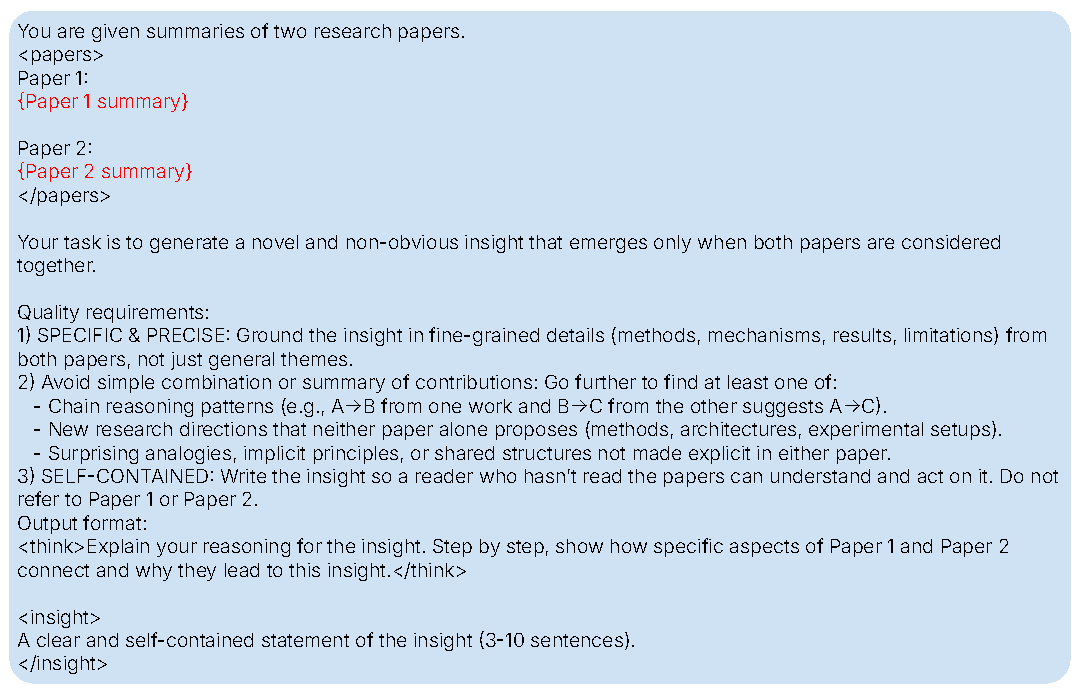
\includegraphics[width=0.95\linewidth]{figs/insight_generation_prompt.pdf}
    % \vspace{-3mm}
    \caption{Prompt for insight generation. The summaries of two parent papers are in \textcolor{red}{red}.}
    \label{fig:insight_generation_prompt}
\end{figure}

\subsection{Ancestor Identification Prompt}
\label{appendix:ancestor_id_prompt}

Here, we present the prompt designed for the ancestor identification task. The primary objective of this prompt is to instruct the model to determine the most influential parent papers for a given downstream target paper. By providing the model with the abstract or conceptual context of the downstream paper, the prompt asks the model to trace the scientific lineage backward and reliably identify which prior works from a candidate pool served as its direct conceptual ancestors.

\begin{figure}[tb]
    \centering
    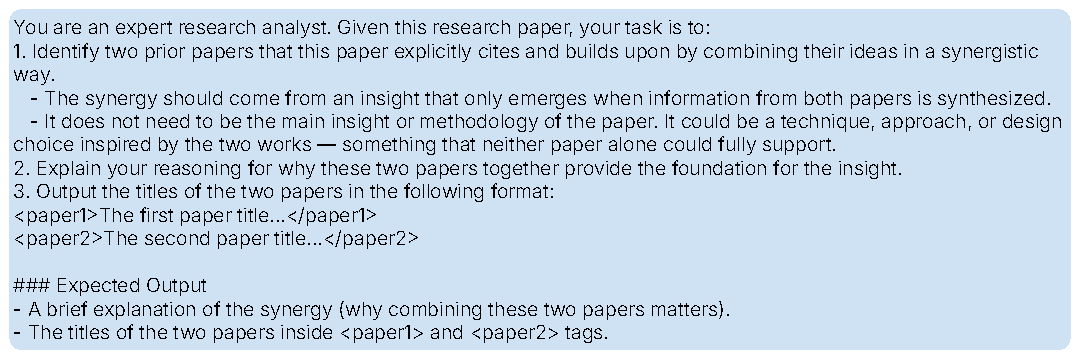
\includegraphics[width=\linewidth]{figs/upstream_citation_prompt.pdf}
    \vspace{-3mm}
    \caption{Prompt for identifying two parent papers whose ideas are synergistically combined to produce the given paper's key insight, which is extracted as the ground-truth target $y^*$.}
    \label{fig:upstream_citation_prompt}
\end{figure}

\subsection{Similarity Judge Prompt}
\label{appendix:similarity_judge_prompt}

Below, we outline the prompt used for automated evaluation and reward scoring via an LLM-as-a-judge framework. To quantitatively assess the quality and relevance of our generated insights, this prompt provides the evaluator model with both the human-verified ground-truth insight and the corresponding model-generated insight. The model is then instructed to critically compare the two texts and output a similarity assessment, evaluating them on semantic alignment, scientific coherence, and the degree of conceptual overlap.

\begin{figure}[t]
    \centering
    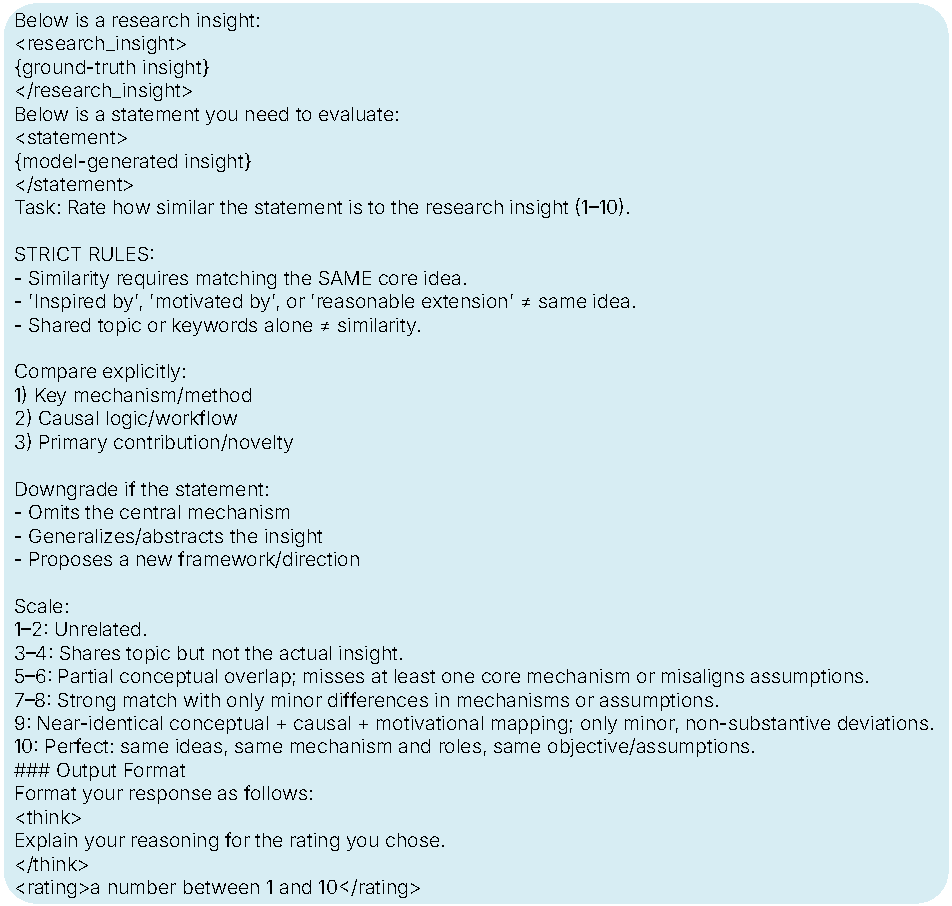
\includegraphics[width=0.6\linewidth]{figs/similarity_judge_prompt.pdf}
    % \vspace{-3mm}
    \caption{Prompt for assessing the similarity between the ground-truth insight and model-generated insight.}
    \label{fig:similarity_judge_prompt}
\end{figure}

\subsection{Rewriting Insight Prompt}
\label{appendix:rewriting_insight_prompt}

To ensure the generated insights could be evaluated consistently, we employed a rewriting step to standardize their format. Figure \ref{fig:rewrite_insight_prompt} displays the prompt used to instruct the model to rewrite the raw insight into a clear, standalone statement without losing its original semantic meaning.

\begin{figure}[H]
    \centering
    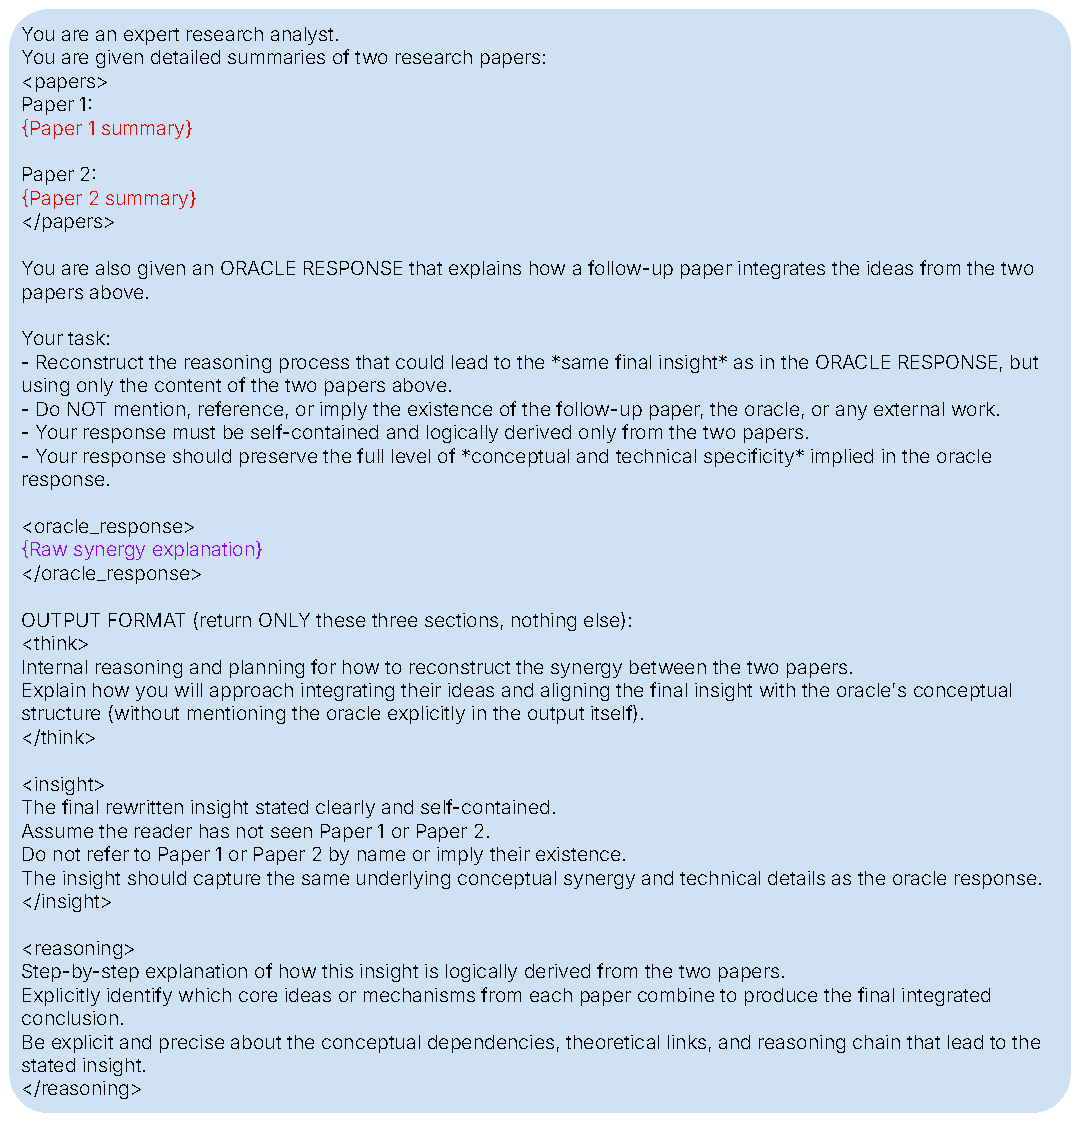
\includegraphics[width=0.6\linewidth]{figs/rewrite_insight_prompt.pdf}
    % \vspace{-3mm}
    \caption{Prompt for rewriting the insight as a standalone statement.}
    \label{fig:rewrite_insight_prompt}
\end{figure}

% \subsection{Similarity Judge Prompt}
% \label{appendix:similarity_judge_prompt}
% \begin{figure}[H]
%     \centering
%     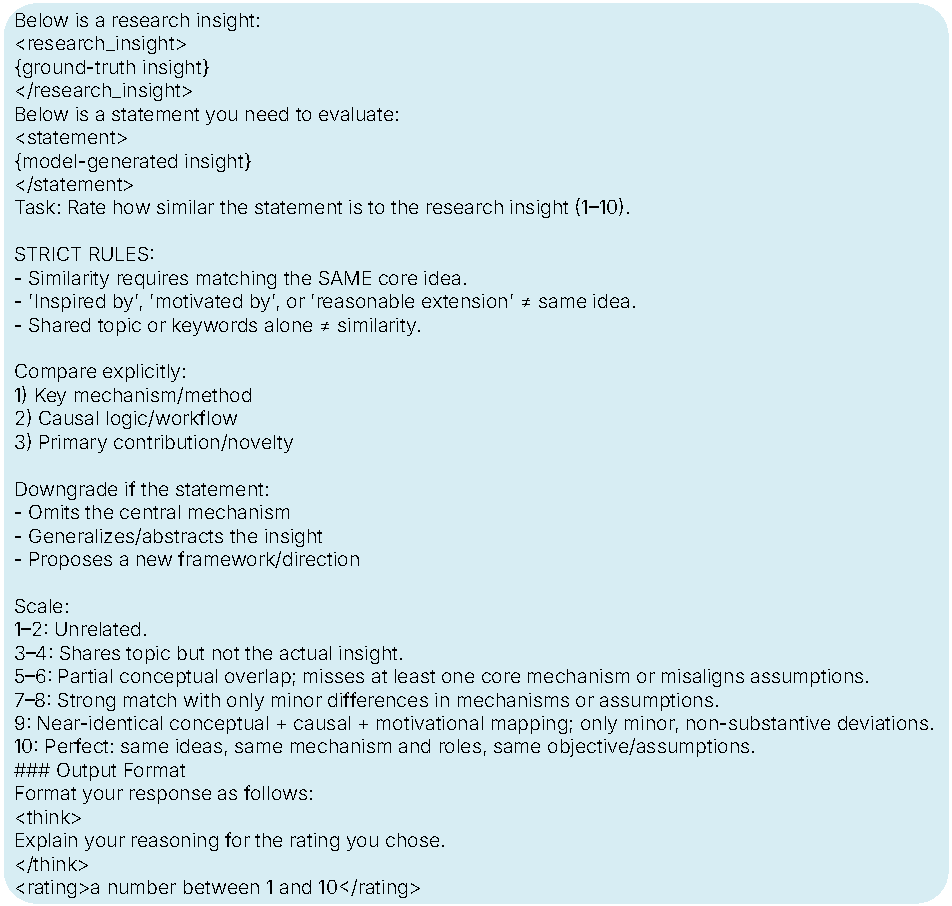
\includegraphics[width=\linewidth]{figs/similarity_judge_prompt.pdf}
%     % \vspace{-3mm}
%     \caption{Prompt for assessing the similarity between the ground-truth insight and model-generated insight.}
%     \label{fig:similarity_judge_prompt}
% \end{figure}

\subsection{Hyperparameters for \ourmethod{} and Baselines}
\label{app:hyperparameters}

We detail the optimization and training configurations used for evaluating \ourmethod{} against the baselines below. The hyperparameter choices were guided by standard practices for aligning large language models, with slight adjustments made to accommodate our specific sequence lengths and batch sizes.

\paragraph{RL Hyperparameters.} 
Table \ref{tab:rl_hyperparameters} outlines the configuration used during the reinforcement learning phase, specifically utilizing the GRPO algorithm. We applied a conservative KL penalty to prevent the model from drifting too far from the reference policy.

\begin{table*}[h]
\centering
\small
\setlength{\tabcolsep}{10pt}
\renewcommand{\arraystretch}{1.15}
\begin{tabularx}{\linewidth}{>{\raggedright\arraybackslash}X >{\centering\arraybackslash}p{0.34\linewidth}}
\toprule
\textbf{Hyperparameter} & \textbf{Value} \\
\midrule
Algorithm                           & GRPO~\citep{shao2024deepseekmath} \\
Training steps                      & 400 \\
Train batch size                    & 64 \\
Group size                          & 8 \\
Max prompt length                   & 3000 \\
Max response length                 & 1296 \\
Learning rate                       & $1\times10^{-6}$ \\
Entropy coefficient                 & 0.001 \\
KL loss coefficient                 & 0.001 \\
KL loss type                        & \texttt{low\_var\_kl} \\
Sampling temperature (train / val)  & 0.6 / 0.6 \\
Samples per prompt (train / val)    & 16 / 8 \\
Max batched tokens                  & 32768 \\
Uneven Clipping (low / high)        & 0.2 / 0.5 \\
\bottomrule
\end{tabularx}
\caption{Key reinforcement learning hyperparameters used in our experiments.}
\label{tab:rl_hyperparameters}
\end{table*}

\paragraph{Supervised Learning Hyperparameters.}
Table \ref{tab:sft_hyperparameters} details the setup for our supervised fine-tuning (SFT) baselines. Where multiple values were explored during our grid search, the final selected optimal configuration is marked in bold.

\begin{table*}[h]
\centering
\small
\setlength{\tabcolsep}{10pt}
\renewcommand{\arraystretch}{1.15}
\begin{tabularx}{\linewidth}{>{\raggedright\arraybackslash}X >{\centering\arraybackslash}p{0.34\linewidth}}
\toprule
\textbf{Hyperparameter} & \textbf{Value} \\
\midrule
Algorithm                           & SFT~\cite{} \\
Epochs                              & 10 \\
Train batch size                    & 64 \\
Max length (input + output)         & 16384 \\
Learning rate                       & $5\times10^{-5}$, $1\times10^{-5}$, \textbf{$5\times10^{-6}$}, $1\times10^{-6}$ \\
Weight decay                        & \textbf{$1\times10^{-2}$}, $1\times10^{-4}$ \\
Sampling temperature (train / val)  & 0.6 / 0.6 \\
Learning rate schedule              & Cosine annealing \\
Learning rate warmup ratio          & 0.01 \\
Gradient checkpointing              & True \\
Gradient accumulation steps         & 16 \\
\bottomrule
\end{tabularx}
\caption{Key supervised fine-tuning hyperparameters used in our experiments. Bold indicates the selected configuration when multiple values were explored.}
\label{tab:sft_hyperparameters}
\end{table*}

\section{Ablations with Diverse LM Judges}
\label{appendix:ablations_with_diverse_lm_judges}

\begin{figure}[H]
    \centering
    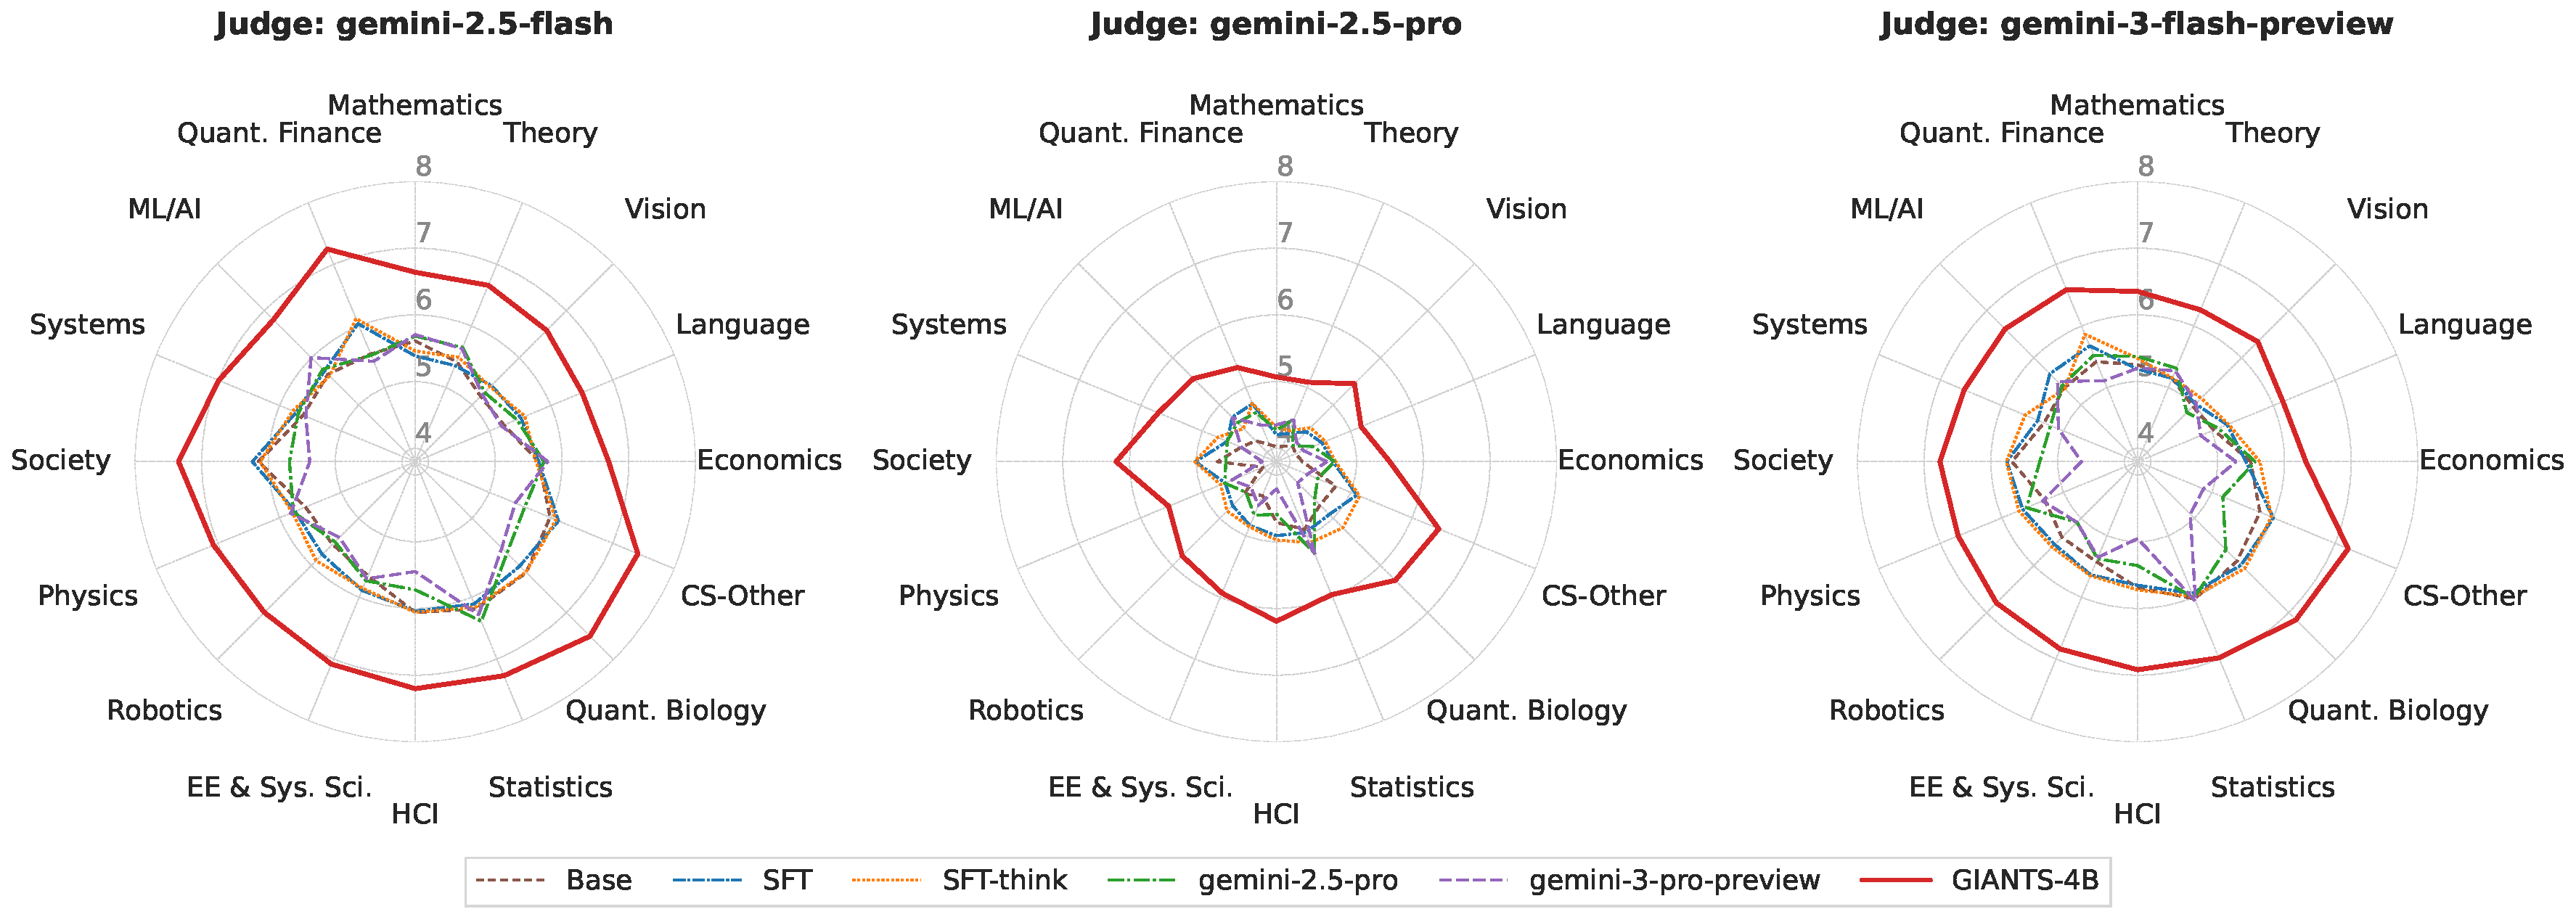
\includegraphics[width=\linewidth]{figs/all_domain_radar_3judges_unseen_parents.pdf}
    \vspace{-3mm}
    \caption{\textbf{Similarity scores on \emph{Test-unseen-parents}}. This is the subset of \ourbenchmark{} test set with only unseen parent papers.}
    \label{fig:all_domain_radar_3judges_unseen_parents}
\end{figure}


\section{Disclosure of LLM Use}
We used an LLM for light editing and revision of the manuscript, assistance with generating figures, and coding support throughout the project.

\section{More Human Eval Details}
\label{app:human_eval}

To validate the reliability of our automated metrics, we conducted a preliminary human evaluation study focusing on insight similarity. Annotators were tasked with scoring the semantic alignment between model-generated insights and ground-truth insights. To facilitate this process and ensure an unbiased environment, we developed a custom web interface, shown in Figure \ref{fig:placeholder}. Importantly, the human annotators were provided with the exact same scoring rubric and guidelines that were given to the LLM judge, allowing us to accurately measure the consistency between human judgment and our automated evaluation pipeline, with the exact context provided to the LLM judge.

\begin{figure}[H]
    \centering
    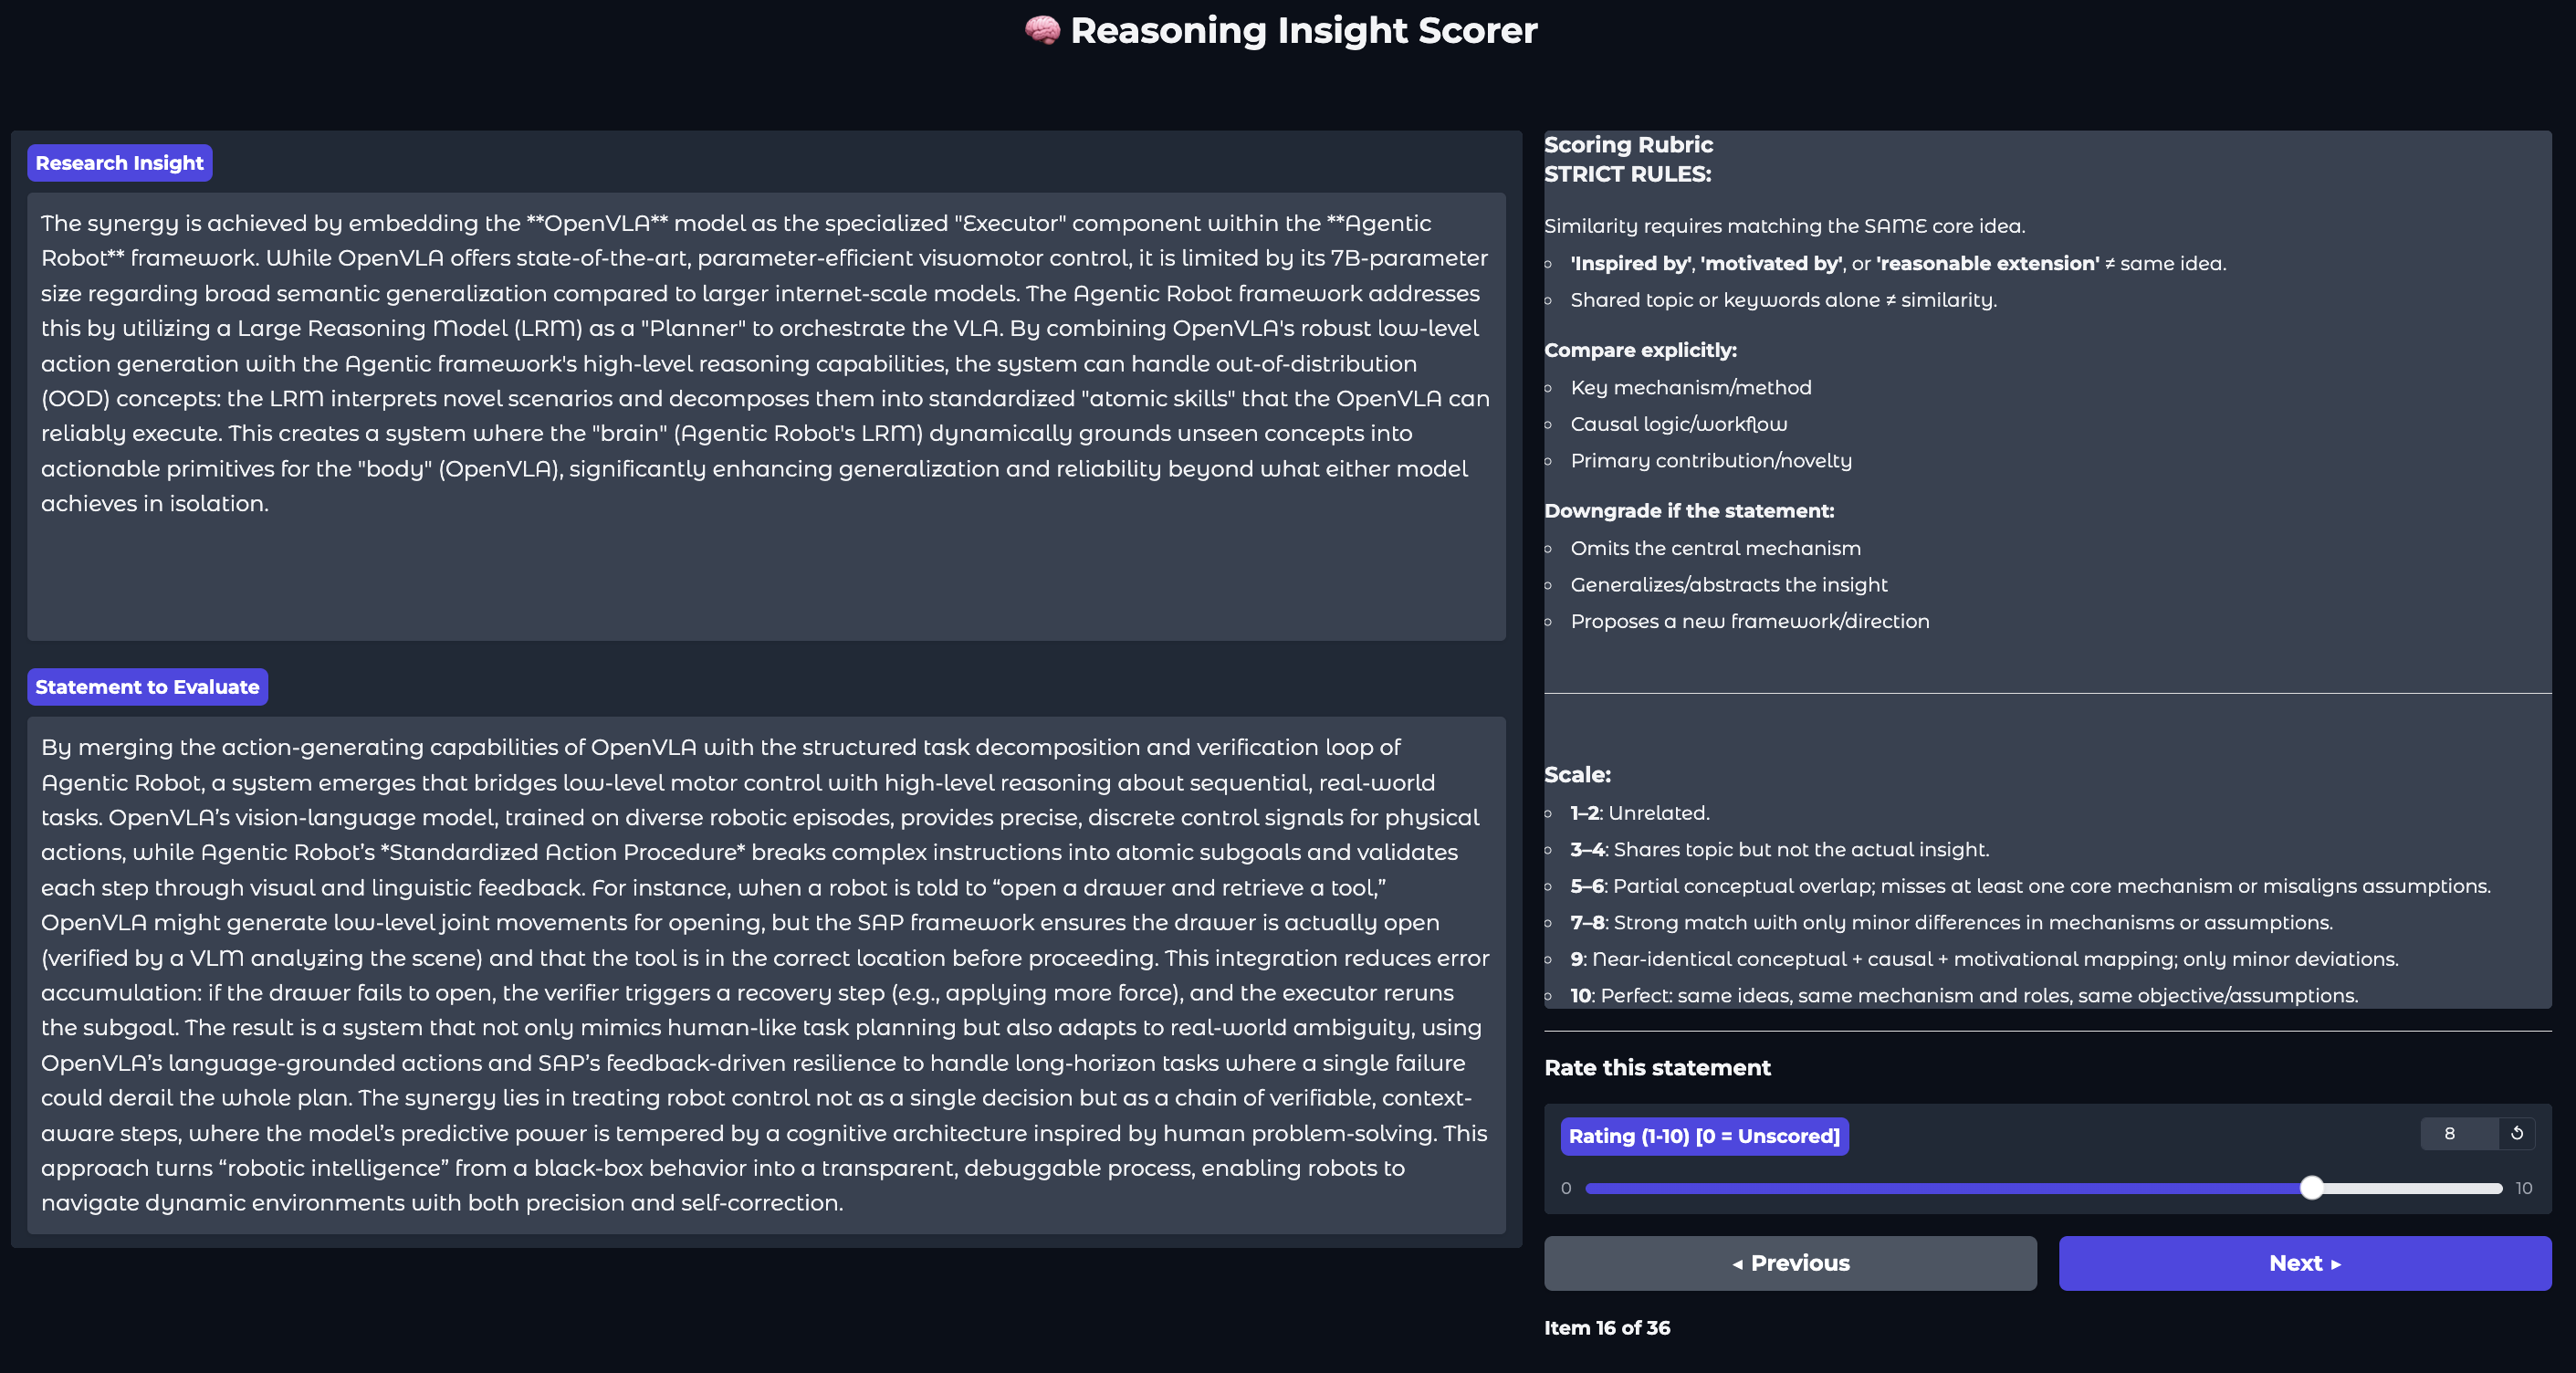
\includegraphics[width=0.8\linewidth]{figs/human_eval.png}
    \caption{\textbf{Human Eval Labeling App} Here is the Gradio interface that was used by human labelers to measure the consistency of LLM similarity with human ratings. The rubric provided to the humans exactly matched that provided to the LLM judge for consistency (with markdown formatting for human interpretability).}
    \label{fig:placeholder}
\end{figure}


\begin{figure}[H]
    \centering
    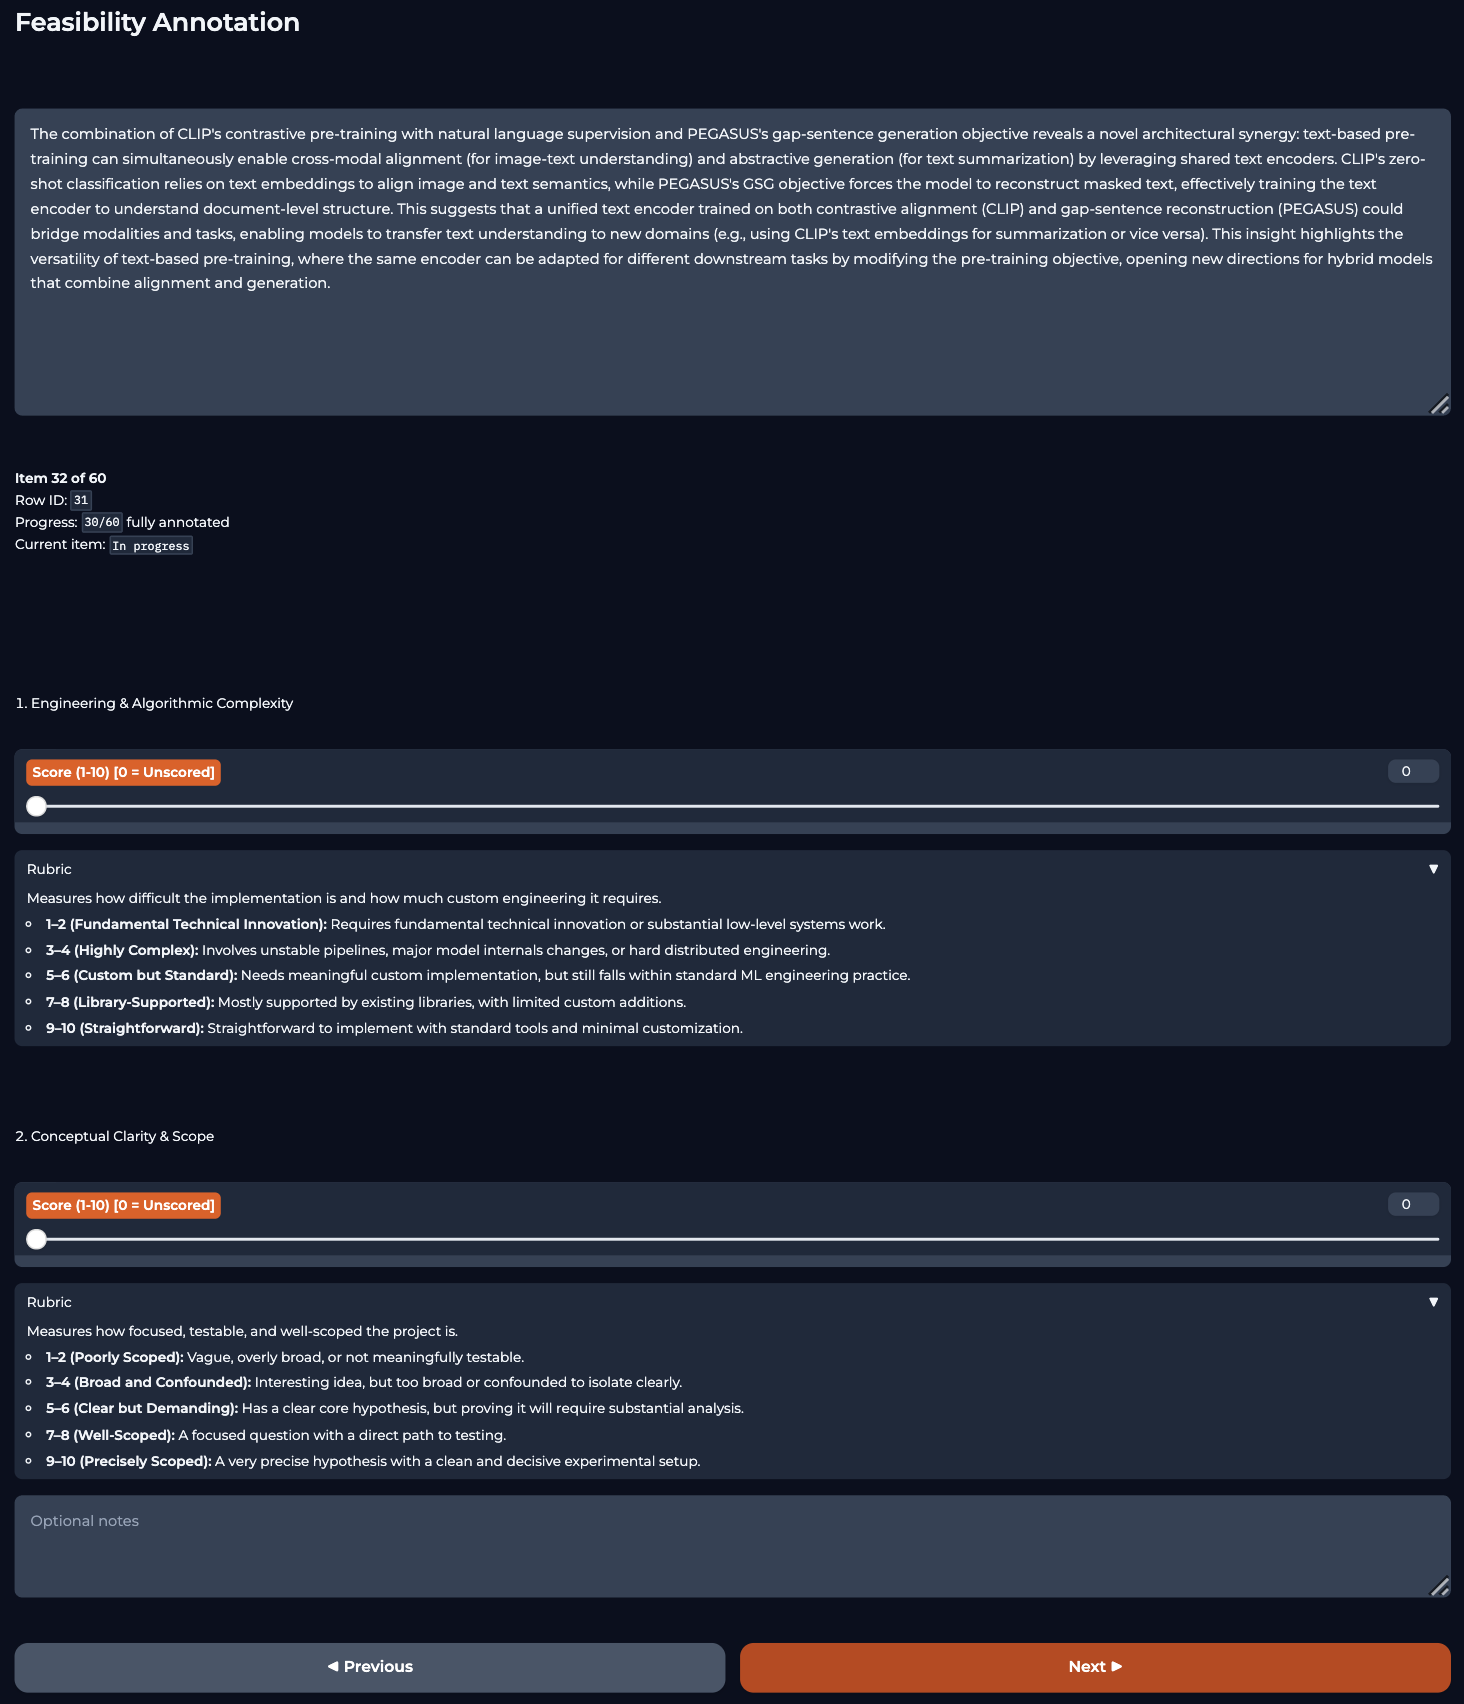
\includegraphics[width=0.8\linewidth]{figs/feasibility_human_eval.png}
    \caption{\textbf{Feasibility Human Eval Labeling App} Here is the Gradio interface that was used by human labelers to measure the feasibility of a research insight with human ratings. The rubric provided to the humans exactly matched that provided to the LLM judge for consistency (with markdown formatting for human interpretability).}
    \label{fig:placeholder}
\end{figure}

